

\subsection{Caso d'Uso: Registrazione di un Nuovo Agente}

Il caso d’uso «Registra nuovo agente» è stato progettato con l’obiettivo di garantire un’esperienza utente fluida e coerente con il resto dell’interfaccia, evitando interruzioni del contesto visivo. Per questo motivo, si è scelto di non introdurre una schermata dedicata, ma di utilizzare una finestra modale (popup), che consente all’utente di eseguire l’operazione senza abbandonare la vista corrente.

\vspace{0.5cm}
\subsubsection{Struttura e Flusso dell’Interazione}
L’interazione si articola in più fasi, guidando l’utente in modo progressivo e controllato:
\begin{itemize}
	\item \textbf{Popup iniziale}: contiene un form per l’inserimento dei dati anagrafici e professionali dell’agente, accompagnato da un unico pulsante in calce con etichetta «Registra nuovo utente».
	\item \textbf{Conferma dell’operazione}: al clic sul pulsante, viene mostrato un \textit{dialog} di doppia conferma per ridurre il rischio di azioni involontarie. I pulsanti di conferma e annullamento sono caratterizzati da colori neutri, in modo da distinguerli visivamente dall’azione primaria dell’applicazione.
	\item \textbf{Feedback di caricamento}: dopo la conferma, il sistema mostra una barra di avanzamento stilizzata con i colori istituzionali del sito. Anche nei casi in cui l’operazione risulti immediata, la barra può essere mantenuta visibile per una breve durata, al fine di fornire un riscontro percettivo chiaro e rassicurante \cite{nielsen1995}.
\end{itemize}

\vspace{0.5cm}
\subsubsection{Messaggio di Conferma e Gestione delle Credenziali}
Al completamento del processo di registrazione, il sistema visualizza un messaggio di successo che informa l’utente dell’avvenuta generazione delle credenziali di accesso.
Il pulsante contestuale assume l’etichetta \textbf{«Copia credenziali»}, permettendo di salvare in modo sicuro i dati generati.
Per prevenire la perdita delle credenziali, la chiusura del dialog è temporaneamente disabilitata fino a quando l’utente non conferma l’avvenuta copia.

\vspace{0.5cm}
\subsubsection{Visualizzazione e Sicurezza dei Dati}
In linea con i principi di \textbf{minimizzazione dei dati} e \textbf{sicurezza dell’informazione} \cite{wickens2008}, la visualizzazione completa delle credenziali non è obbligatoria:
il sistema privilegia la protezione dei dati sensibili, evitando di esporre informazioni in chiaro nell’interfaccia.
In alternativa, è possibile prevedere una versione mascherata delle credenziali o la sola visualizzazione di elementi non sensibili, mantenendo comunque la trasparenza informativa per l’utente.
\begin{figure}[H]
	\centering
	\begin{tikzpicture}[node distance=1.5cm and 1cm, auto]
		% Nodo per immagine 1 con didascalia sotto
		\node (img1) {
			\begin{tabular}{c}
				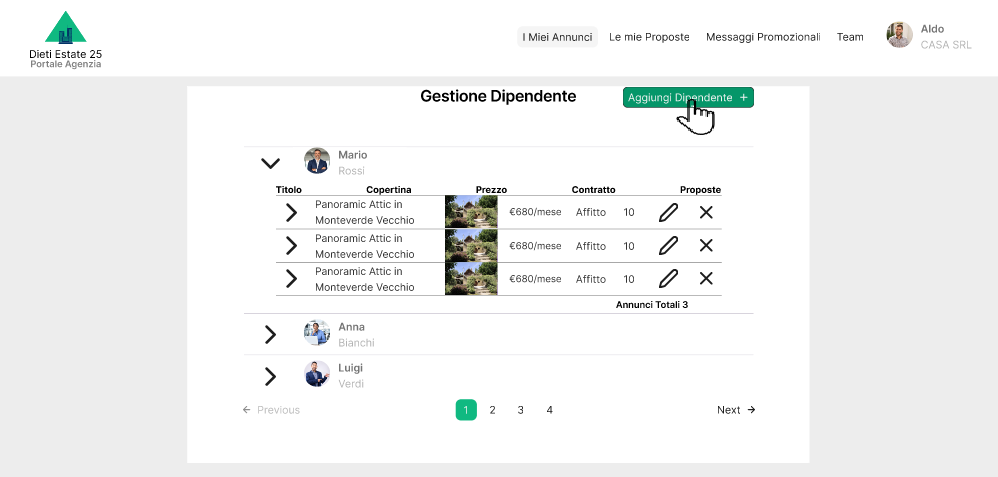
\includegraphics[width=0.7\textwidth]{Immagini/Mockup/nuovoAgente/scenario principale/clickNuovoDipendente.png} \\
				Cockburn: step 1
			\end{tabular}
		};
		
		% Nodo per immagine 2 con didascalia sotto, posizionato a destra di img1
		\node (img2) [below=of img1] {
			\begin{tabular}{c}
				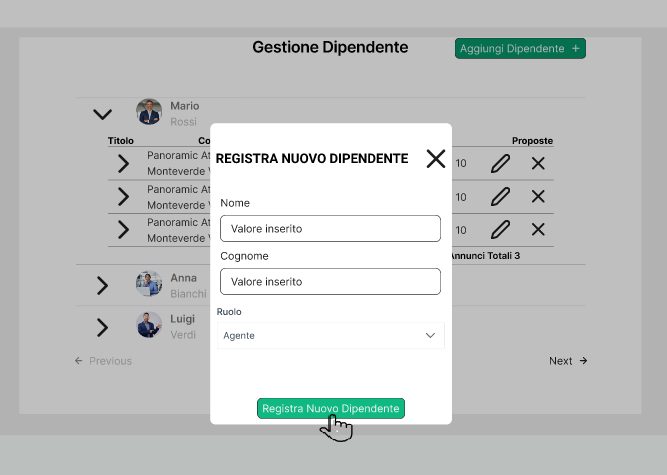
\includegraphics[width=0.7\textwidth]{Immagini/Mockup/nuovoAgente/scenario principale/clickFormNuovoAgente.png} \\
				Cockburn: step 2/3/4
			\end{tabular}
		};
		
		% Nodo per immagine 3 con didascalia sotto, posizionato sotto img2
		\node (img3) [below=of img2] {
			\begin{tabular}{c}
				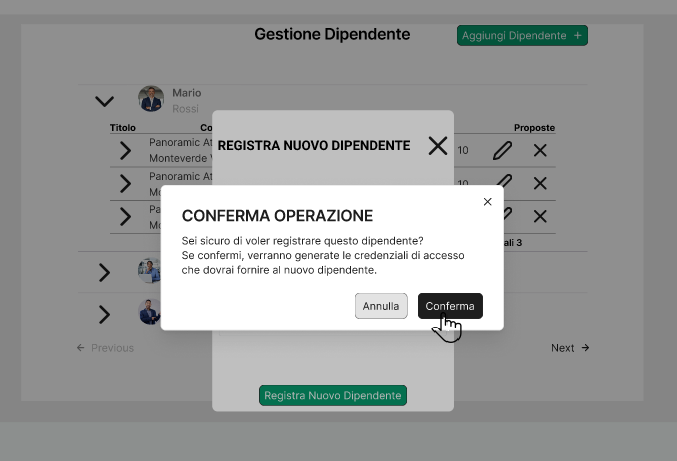
\includegraphics[width=0.7\textwidth]{Immagini/Mockup/nuovoAgente/scenario principale/ClickAllertConferma.png} \\
				Cockburn: step 5/6
			\end{tabular}
		};
		
		% Disegna le frecce
		\draw[->, thick] (img1) -- (img2);
		\draw[->, thick] (img2) -- (img3);
		
	\end{tikzpicture}
	\caption{Mockup: scenario principale della tabella di Cockburn del caso d'uso: Registra nuovo agente.}
	\label{fig:tikz_flow}
\end{figure}

\newpage

\begin{figure}[H]
	\centering
	\begin{tikzpicture}[node distance=1.5cm and 1cm, auto]
		% Nodo per immagine 1 con didascalia sotto
		\node (img1) {
			\begin{tabular}{c}
				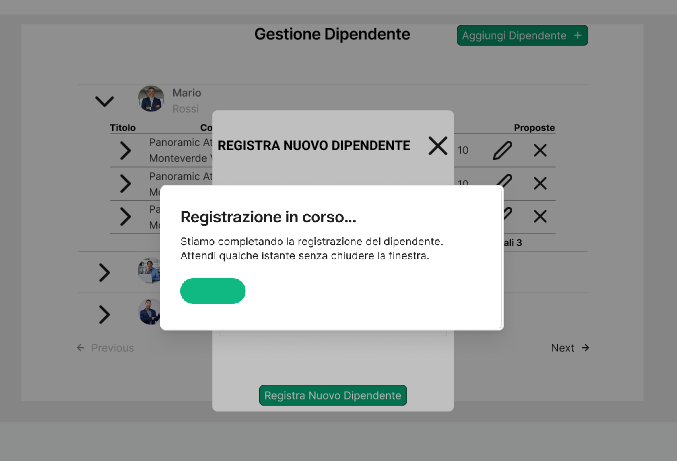
\includegraphics[width=0.7\textwidth]{Immagini/Mockup/nuovoAgente/scenario principale/caricamentoRegistrazione.png} \\
				Cockburn: step 6/7/9
			\end{tabular}
		};
		
		% Nodo per immagine 2 con didascalia sotto, posizionato a destra di img1
		\node (img2) [below=of img1] {
			\begin{tabular}{c}
				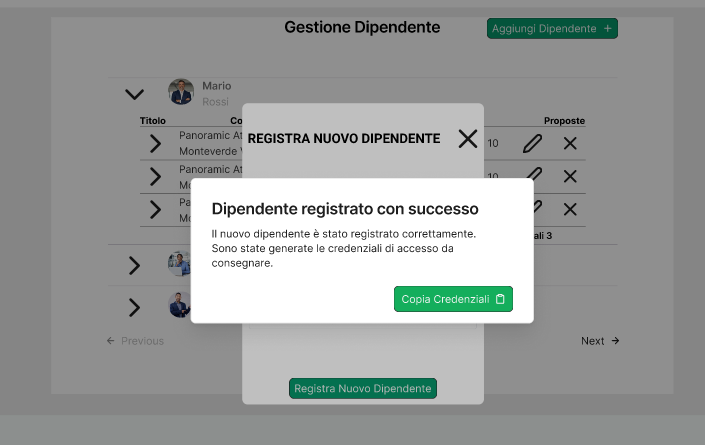
\includegraphics[width=0.7\textwidth]{Immagini/Mockup/nuovoAgente/scenario principale/allertRegistrazioneEffettuata.png} \\
				Cockburn: step 10
			\end{tabular}
		};
		
		% Nodo per immagine 3 con didascalia sotto, posizionato sotto img2
		\node (img3) [below=of img2] {
			\begin{tabular}{c}
				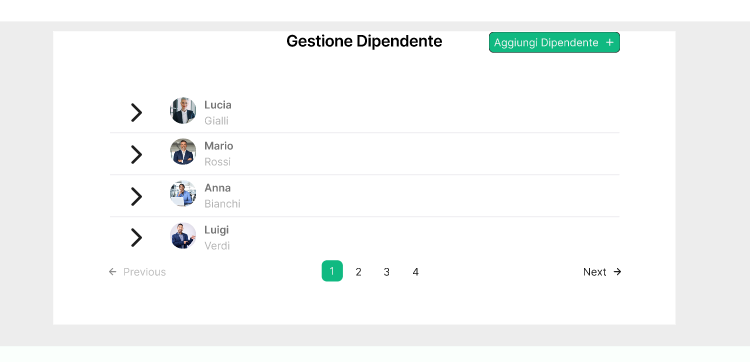
\includegraphics[width=0.7\textwidth]{Immagini/Mockup/nuovoAgente/scenario principale/visualizzazioneNuovaRegistrazione.png} \\
				Cockburn: step 11
			\end{tabular}
		};
		
		% Disegna le frecce
		\draw[->, thick] (img1) -- (img2);
		\draw[->, thick] (img2) -- (img3);
		
	\end{tikzpicture}
	\caption{Mockup: scenario principale della tabella di Cockburn del caso d'uso: Registra nuovo agente.}
	\label{fig:tikz_flow}
\end{figure}

\newpage

\subsubsection{Estensione A: Campi Non Compilati o Compilati Erroneamente}

Durante la procedura di registrazione di un nuovo agente, il manager potrebbe tentare di completare l’operazione senza aver inserito tutti i dati richiesti o compilando alcuni campi in modo errato.
Per prevenire errori di input e garantire la coerenza delle informazioni salvate nel sistema, è previsto un controllo di validazione lato client.

\subsubsection{Gestione del Messaggio di Errore}
Nel momento in cui il manager clicca su \textbf{“Registra dipendente”} con uno o più campi incompleti o non validi, il sistema intercetta l’errore e mostra un messaggio specifico sotto ciascun campo non conforme.
Il messaggio indica chiaramente la tipologia di errore (es. campo obbligatorio, formato non valido, valore numerico errato), fornendo un feedback immediato e mirato.

L’interfaccia rimane attiva e consente al manager di correggere i dati direttamente nella stessa schermata, evitando la perdita delle informazioni già inserite.
Una volta completate le correzioni, il manager può ripetere l’operazione di registrazione, tornando così al flusso principale dello scenario (Step 3).

Questa soluzione progettuale segue i principi della \textbf{visibilità dello stato del sistema} e della \textbf{prevenzione degli errori} \cite{nielsen1995}, migliorando la comprensibilità e riducendo la frustrazione dell’utente.

\begin{figure}[H]
	\centering
	\begin{tikzpicture}[node distance=1.5cm and 1cm, auto]
		% Nodo per immagine 1 con didascalia sotto
		\node (img1) {
			\begin{tabular}{c}
				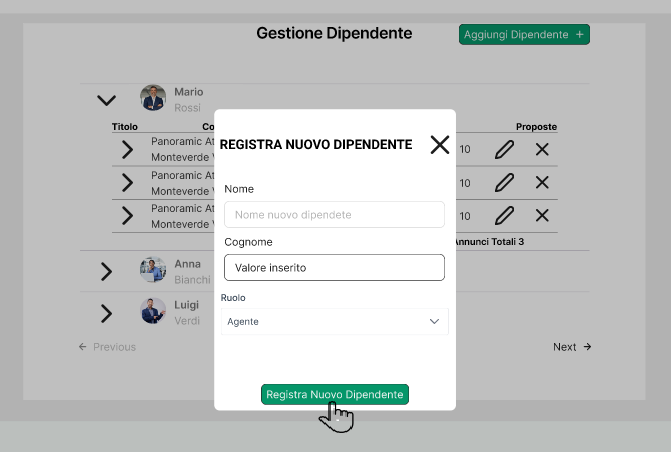
\includegraphics[width=0.7\textwidth]{Immagini/Mockup/nuovoAgente/extension A/nomeNonInserito.png} \\
				Cockburn: step 4.A
			\end{tabular}
		};
		
		% Nodo per immagine 2 con didascalia sotto, posizionato a destra di img1
		\node (img2) [below=of img1] {
			\begin{tabular}{c}
				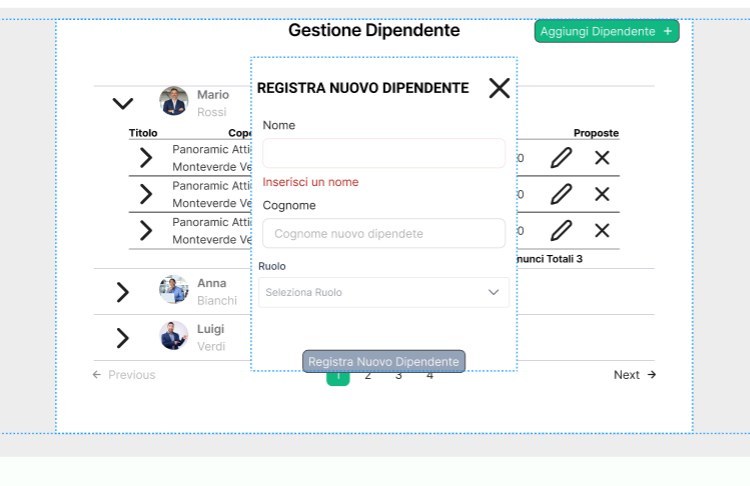
\includegraphics[width=0.7\textwidth]{Immagini/Mockup/nuovoAgente/extension A/messaggioDiErrore.png} \\
				Cockburn: step 5.A
			\end{tabular}
		};
	
		
		% Disegna le frecce
		\draw[->, thick] (img1) -- (img2);
		
	\end{tikzpicture}
	\caption{Mockup: Extension A della tabella di Cockburn del caso d'uso: Registra nuovo agente.}
	\label{fig:tikz_flow}
\end{figure}



\subsubsection{Estensione B: Nome e Cognome già Registrati}

Nel caso in cui il manager tenti di registrare un agente con nome e cognome già presenti nel sistema, viene eseguito un controllo automatico per evitare la duplicazione dei profili e garantire l’univocità dei dati.

\subsubsection{Gestione del Conflitto e Generazione dell’Email Alternativa}
Dopo aver cliccato su \textbf{“Conferma”}, il sistema mostra una breve fase di caricamento e verifica l’esistenza di un profilo con lo stesso nome e cognome.
In caso di corrispondenza, il sistema genera automaticamente un’email alternativa che include un identificativo univoco, assicurando così la distinzione tra gli utenti.

Completata la procedura, il sistema ritorna al passo 9 dello scenario principale e la registrazione viene finalizzata correttamente.
Questa soluzione applica il principio della \textbf{gestione flessibile degli errori}, consentendo di proseguire l’operazione senza interruzioni e mantenendo la consistenza dei dati.




\subsubsection{Estensione C: Annullamento della Registrazione nella Finestra di Conferma}

Nel caso in cui, all’interno della finestra di conferma, il manager scelga di annullare la registrazione, il sistema interrompe il processo evitando la creazione di un nuovo agente.

\subsubsection{Comportamento del Sistema}
Se il manager clicca su \textbf{“Annulla”} invece di confermare l’operazione, la finestra di dialogo viene chiusa e il flusso ritorna al passo 3 dello scenario principale, consentendo di modificare i dati inseriti o abbandonare la procedura.

Questa interazione segue il principio del \textbf{controllo da parte dell’utente} \cite{nielsen1995}, garantendo la possibilità di interrompere o correggere un’azione prima che diventi definitiva.
\subsubsection{Estensione D: Mancata Connessione al Sistema}

In alcune circostanze, il manager potrebbe non riuscire a completare la registrazione a causa di problemi di connessione o di un temporaneo malfunzionamento del server.
Il sistema gestisce questa evenienza fornendo un chiaro feedback sull’esito negativo dell’operazione.

\subsubsection{Gestione dell’Errore di Connessione}
Dopo aver cliccato su \textbf{“Conferma”}, il sistema mostra un breve stato di caricamento.
Se la connessione al server non riesce, viene visualizzato un pop-up di allerta che informa l’utente dell’impossibilità di completare la registrazione per motivi tecnici.

In questo caso, l’\textbf{use case è considerato fallito}, ma il manager può chiudere il messaggio e riprovare l’operazione una volta ristabilita la connessione.
Questa soluzione si basa sui principi di \textbf{visibilità dello stato del sistema} e di \textbf{recuperabilità dall’errore}, assicurando chiarezza e prevedibilità anche in situazioni di errore tecnico.
\begin{figure}[H]
	\centering
	\begin{tikzpicture}[node distance=1.5cm and 1cm, auto]
			% Nodo per immagine 3 con didascalia sotto, posizionato sotto img2
		\node (img1){
			\begin{tabular}{c}
				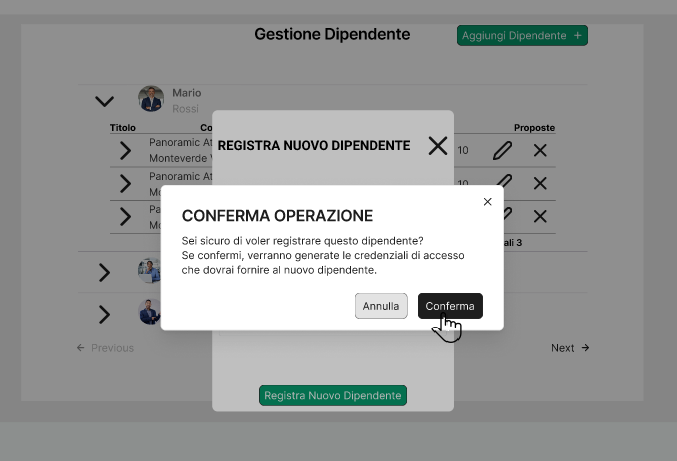
\includegraphics[width=0.7\textwidth]{Immagini/Mockup/nuovoAgente/scenario principale/ClickAllertConferma.png} \\
				Cockburn: step 6.D
			\end{tabular}
		};
		
		% Nodo per immagine 1 con didascalia sotto
		\node (img2)  [below=of img1] {
			\begin{tabular}{c}
				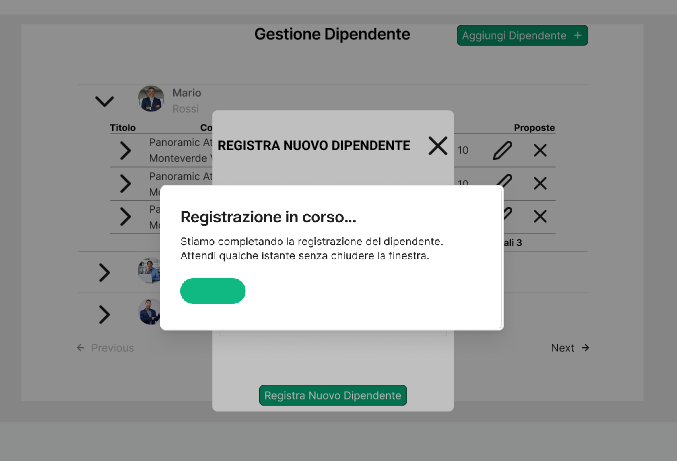
\includegraphics[width=0.7\textwidth]{Immagini/Mockup/nuovoAgente/scenario principale/caricamentoRegistrazione.png} \\
				Cockburn: step 7.D
			\end{tabular}
		};
		
		% Nodo per immagine 3 con didascalia sotto, posizionato sotto img2
		\node (img3) [below=of img2] {
			\begin{tabular}{c}
				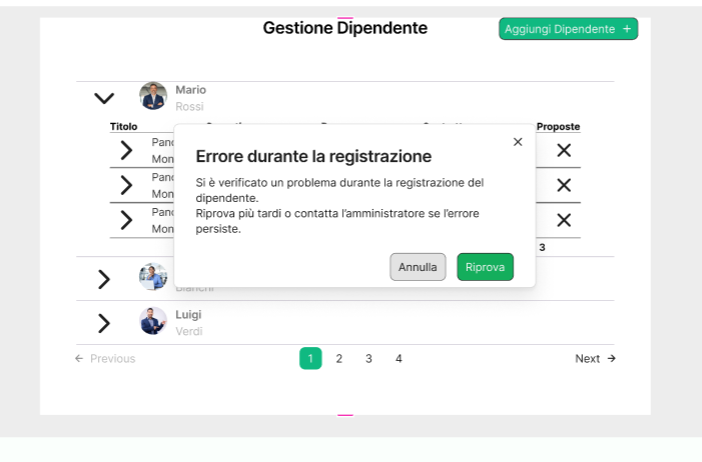
\includegraphics[width=0.7\textwidth]{Immagini/Mockup/nuovoAgente/extension D/messaggioDiErrore.png} \\
				Cockburn: step 8.D
			\end{tabular}
		};
		
		% Disegna le frecce
		\draw[->, thick] (img1) -- (img2);
		\draw[->, thick] (img2) -- (img3);
		
	\end{tikzpicture}
	\caption{Mockup: Extension D della tabella di Cockburn del caso d'uso: Registra nuovo agente.}
	\label{fig:tikz_flow}
\end{figure}
